\chapter{Sire Indexes}
\label{cha:Lush_Chapter_31}
\index{Progeny test|(}
\index{Sire indexes|(}

A sire index is a way of expressing what the sire's progeny indicate
about his heredity. It is most needed for characteristics which the sire
cannot show himself: milk and fat production in dairy cattle, egg production
in poultry, prolificacy in swine and sheep, nursing ability in all
mammals, and certain traits of disposition which are expressed differently
in males and females,\footnote{Hammond, John, 1932, \textit{Report on
Cattle-breeding in Jamaica and Trinidad}, Publication No. 58 of the Empire
Marketing Board, London.} etc. For characteristics which the sire can
manifest in himself, a sire index is useful for revising estimates of his
hereditary value when such estimates have been based only on his own
characteristics and on his pedigree.

A complete sire index would logically be based on all available
information about the sire's own characteristics and about his ancestors
and collateral relatives, as well as on the information about his progeny;
but most of the current discussion about sire indexes deals only with
ways to use the information about the progeny and their other parents.
Sire indexes of that kind are only special applications of the principle
of the progeny test discussed in chapter 15. Sire indexes are mentioned
most often in writings on dairy and poultry breeding.\footnote{See
\textit{Jour. of Dy. Sci.}, 16:501--22, for a discussion of the general
principles involved.} The wording used in the rest of this chapter applies
primarily to dairy cattle. The principles are the same in other cases, but
the importance of some of the considerations may change.

\section*{THEORETICAL BASIS}
\index{Sampling nature of inheritance|(}

The reasons for computing a sire's index as $2D - M$, when \textit{D} is
the average of his daughters and \textit{M} is the average of the dams of
those daughters, may be seen from the equations on page \pageref{eqn-page-198}.
The reasons for not trusting the index completely arise from what are called
``Mendelian errors'' and ``errors of appraisal'' in those equations.

The Mendelian errors come from chance at segregation which permits
gametes coming from the same parent to contain different genes,
so that some offspring are genetically better than the average of their
parents while others are worse. These variations are truly random, provided
the daughters are an unselected sample. Therefore, they tend to
cancel each other and their importance in an average diminishes as the
number of daughters increases.

The errors of appraisal come from the fact that even after we have
corrected the record of a daughter or a dam for age, for times milked
per day, and for every other non-standard environmental circumstance
about which we know, the record will be higher in some cases and lower
in others than corresponds to the real breeding value of the cow. Such
of these errors as are random tend to diminish in importance as the
number of daughters in the average increases, just as the Mendelian
errors do. Some of the errors of appraisal are not random but tend to be
in the same direction for all the daughters or for all the mates of the
same bull but may be in a different direction or be different in size for
the daughters or mates of other bulls. They may even be different for
the daughters and for the mates of the same bull. Frequent causes of
these biased errors are: (1) The general level of environment to which
each group of daughters or of dams was exposed may have varied much
from one group to another and we may not know what the environment
was in each case, or may know it but not be able to allow perfectly for
its effects. (2) The daughters or the records which were used to represent
them may have been selected ones, rather than a fair sample of all.
(3) The dams of these daughters may have been a selected group and
the intensity of that selection, too, may have varied from one sire to
another. Such biased errors do not tend to cancel each other as the
number of daughters increases.

The actual numerical value of each sire index is partly determined
by the real breeding value of the sire but partly also by whatever biased
errors that index contains and by the uncanceled remainder of the random
errors. Accordingly sire indexes will vary more than the real breeding
values of the sires do. The sires with the very highest indexes are
generally good sires but they are not likely to be as good as their
indexes. Similarly the sires with low indexes are generally poor sires
but they are not usually as poor as their indexes. We shall make the
smallest mistakes if we estimate the breeding value of each sire at part
way between his index and the average of his breed.
\index{Sampling nature of inheritance|)}

The principles governing how much confidence the index deserves
can best be understood by considering first the dependability of an
index (\textit{I}) based on the record of only one daughter (\textit{D})
and her dam (\textit{M}). The variance of \textit{D} and of \textit{M}
will be nearly the same. For clarity in the argument this variance can
be divided into the additively genetic portion (\textit{G}) plus a portion
(\textit{E}) due to random discrepancies between the genetic value and and
the record of the cow, plus a portion (\textit{C}) due to those
discrepancies between record and breeding value which are alike for all
the daughters of a bull or for all the mates of a
\newpage
\noindent
bull. Then, according to the usual formula for the variance of a difference,
the variance of the index is:

\[ 5G + 5C + 5E - 2G - 4xC = 3G + (5 - 4x)C + 5E \]

\noindent
where \textit{x} is the correlation between \textit{C} for a daughter and
\textit{C} for her dam. The sire's breeding value is responsible for only
\textit{G} of the variance in this index, as may be seen by referring to
diagram \textit{B} in Figure 32. That diagram shows how the genetic value
of an individual is \nicefrac{1}{4} determined by the genetic value of its
sire, \nicefrac{1}{4} by the genetic value of its dam and \nicefrac{1}{2}
by chance at Mendelian segregation.\footnote{If sire or dam were inbred,
the fraction determined by the genetic value of that parent would be
$\dfrac{1+F}{4}$, while correspondingly less part would be determined by
chance at segregation. In most populations inbreeding is unusual and is so
mild that we can ignore it here with little error.} The genetic variance
which the dam determines is removed in subtracting \textit{M} from
\textit{2D}. That leaves in the variance of \textit{I} only \textit{3G}
of the \textit{4G} which is the genetic variance in \textit{2D}. The sire
is responsible for \nicefrac{1}{3} of that \textit{3G}, while chance at
segregation is responsible for \textit{2G}.

When the index is based on n daughter-dam pairs, instead of one,
the random parts of the variance in \textit{I} become only
\nicefrac{1}{\textit{n}} as large. Thus the variance of \textit{I}
based on \textit{n} pairs is: $G + (5 - 4x)C + (2G + 5E)/n$.
The equation which will predict with the least error the breeding value
of the sire becomes:

\[ Sire - A = \dfrac{n}{n[1 + (5 -4x)C/G] + 2 + 5E/G}(I - A) \]

\noindent
where \textit{A} is the breed average. The fraction in this equation can be
considered as showing the extent to which the index should be believed.
The square root of this fraction is the correlation between the index
and the real breeding value of a bull.

\index{Heritability|(}
Wright has discussed this equation for the case of complete heritability;
i.e., when \textit{C} and \textit{E} are both zero. Then it becomes simply:
\(Sire - A = \dfrac{n}{n + 2}(I - A)\) and confidence in the index becomes almost
complete when the number of daughter-dam pairs is much more than
five. This, however, is not very realistic because in practice \textit{E} will
always be real and for many characteristics it will be much larger than
\textit{G}. \textit{C} also is likely to have a real value in most sets of data
which are collected from many herds, since it is rarely if ever possible to
discount accurately for all of the differences in management and environment
from one herd to another.

The effects of \textit{E} may be seen most clearly by considering the case in
which \textit{C} is zero but heritability \(\left(i.e., \dfrac{G}{G + E}\right)\) varies.
Then the fraction in the prediction equation becomes: \(\dfrac{n}{n + 2 + 5E/G}\)
which takes values such as the following:

{\renewcommand{\arraystretch}{2}%
\begin{table}[h]
	\centering
	\begin{tabular}{C{2cm}C{1cm}C{2cm}}
	Heritability	& & Fraction			\\
	.10				& & $\dfrac{n}{n + 47}$	\\
	.20				& & $\dfrac{n}{n + 22}$	\\
	.25				& & $\dfrac{n}{n + 17}$	\\
	.33				& & $\dfrac{n}{n + 12}$	\\
	.50				& & $\dfrac{n}{n + 7}$	\\
	.71				& & $\dfrac{n}{n + 4}$	\\
	1.00			& & $\dfrac{n}{n + 2}$
	\end{tabular}
\end{table}}

\noindent
If \textit{E} is large the justifiable confidence in the index is obviously
very low when \textit{n} is small. Nevertheless perfect trust in the index
is approached, although slowly, as \textit{n} becomes extremely large.
\index{Heritability|)}

\index{Regression|(}
The existence of \textit{C} changes the situation so that confidence in the
index increases more slowly with \textit{n} and no longer approaches unity
as a limit. Instead it approaches $1/y$ where $y = I + (5 - 4x)C/G$. This
\textit{y} can be a large number if \textit{C} is large relative to \textit{G}
and if \textit{x} is small. That
$C/G$ may often be as large as 1.0 in dairy data is indicated by correlation
usually of the order of .2 to .3 between the records of unrelated or
slightly related cows kept in the same herd. The general size of \textit{x}
is less certain. It would be 1.0 if all of \textit{C} came from general
differences in environment from herd to herd and if the peculiar environment
of each herd were unchanging, year after year. However, part of \textit{C}
can come from herd environment which changes between the time when the
dams made their records and the time when the daughters made theirs.
A part of \textit{C} can come from selection of the dams or of the daughters
having been more intense for some bulls than for others. Hence \textit{x}
will not be 1.0 although it may usually be above .5. The case $C = G$ and
$x = .5$, which is not unreasonable for dairy data, will illustrate the
power of \textit{C} to limit confidence in the index. In that case confidence
in the index will not exceed \nicefrac{1}{4}, even when the number of daughter-dam
pairs becomes exceedingly large. If \textit{C} is only half as large as
\textit{G}, the corresponding limit is \nicefrac{2}{5}. If \textit{C} is as large
as \textit{G} but \nicefrac{3}{4} of \textit{C} is alike for the daughters and
for the mates of the same bull, the limit is \nicefrac{1}{3}.
\index{Progeny test|)}
\index{Regression|)}

Obviously anything which can be done to diminish \textit{C} and
\textit{E} by keeping the environmental conditions standard and
alike for all daughters and dams, or by correcting the actual
records for the effects of varying environment or of unequal
selection of the mates of various bulls will increase the confidence
which the index deserves.

\section*{PRACTICAL CONSIDERATIONS}

\textsc{Relative rating}. For comparing bulls with one another when all
of them have the same number of daughter-dam pairs, the index is all
that is needed since it will then rank all the bulls in the same order and
proportionately the same distance apart, no matter what is the value of
\textit{C} or \textit{E} or \textit{x}. The need for knowing how much to
regress the indexes toward the breed average arises only when we wish to
compare bulls proven on different numbers of pairs, or when we wish to
compare a bull's index with a cow's record. For the first of these purposes
ignorance of \textit{C}, \textit{E}, and \textit{x} makes only a little
difference unless n varies extremely from one sire to another. Doubling
\textit{n} will double the numerator but only the first part of the
denominator. If that first part of the denominator is already more than
half of it, the doubling of \textit{n} will increase the fraction by less
than one third of its initial value. Hence further increases in \textit{n}
when it is already large add only slightly to the confidence which the index
deserves.

\textsc{Comparing bulls' indexes with cows' records}. The necessity for
comparing a bull's index with the records of a cow is met almost every
time we evaluate a pedigree in which the sire or one or both grandsires
are proven. For example, in choosing between young bulls \textit{A} and
\textit{B} we may find that the sire of \textit{A} has an index which
is 40 pounds higher than the index of \textit{B}'s sire but that the
records of \textit{B}'s dam average 60 pounds higher than the records of
\textit{A}'s dam. To estimate whether \textit{A} or \textit{B} probably
has the higher breeding value, we have to decide whether a difference of
40 pounds in sire indexes is as important as a difference of 60 pounds
in the records of cows. If the cow's record is left in its actual
form, sire indexes can be compared directly and fairly with it if the
indexes have been regressed only enough that they would have about
the same variability as the cows' records -- a little more variability if an
index is generally a bit more accurate as an indicator of a sire's breeding
value than a cow's record is of her breeding value, but a little less
variability if the indexes are generally less accurate. If the indexes are
each numerically equal to the estimated breeding values of the bull to
whom it belongs, then the cow's record also should be regressed far
enough toward the breed average to make it likewise an unbiased estimate
of her breeding value. Present practice in this respect is not uniform.
The Holstein-Friesian Association publishes indexes based on six
or more pairs and does not regress them at all. This makes these indexes
just a bit more variable than the records of cows with one record each.
The same is true of the indexes computed by the American Dairy Cattle
Club from the records published by the Dairy Bureau of the USDA,
except that in this case the minimum number of pairs is five. The Ayrshire
Association since late 1944 has been regressing sire indexes half
way toward the breed average and basing them on at least ten pairs.
Sire indexes regressed this much are only about half as variable as records
of cows who have one lactation each.

\textsc{Number of daughter-dam pairs needed.} From the principles governing
the accuracy of sire indexes it is clear that accuracy is low when
the number of pairs is very small but it is also clear that accuracy does
not suddenly become perfect when a certain number is reached. Instead
the accuracy increases at an ever-decreasing rate as the number rises.
Since the gain from increasing n comes solely from the decrease which
that makes in the term $(2G + 5E)/n$ in the variance of \textit{I}, the
advantages in having \textit{n} any larger have mostly been reaped by the
time $(2G + 5E)/n$ has already become distinctly smaller than $G + (5-4x)C$.
\noclub

Largely by trial and error but partly based on considerations like
these, all official plans for computing indexes specify some minimum
number for \textit{n} before an index will be computed at all. One important
consideration which has kept the minimum numbers small is that if
many daughters were required few bulls could be proved. Those who
made the Dairy Bureau policy thought that the increased accuracy
which the proof would have, if six were required instead of five, would
be more than offset by the fact that the large number of bulls who have
only five comparisons would thereby not be brought to the attention of
breeders who might otherwise hear of them and make some use of that
information. There is good reason for believing this still to be sound
policy, although the original decision was made years ago. One suggestion
for reaping both advantages is that bulls be given a preliminary
index when five pairs are available and another index when the number
has risen to another level, for example eight or ten. The Ayrshire
Association does something of this kind. This, however, adds to the
bookkeeping and some customers will not distinguish between the bulls
with only preliminary proof and the bulls with more complete proof.

\textsc{Simplicity} of the index is important for explaining
it to the potential users and giving them the proper amount of confidence
in it, for ease and speed of computing it, and to reduce the chance of
clerical errors. Yet the underlying principles are such that at least a
little accuracy must be sacrificed if simplicity is to be achieved in data
in which \textit{n} varies or if the same index is to be used in different
populations, such as Dairy Herd Improvement Associations or Herd Improvement
Registry, in which the relative proportions of \textit{G}, \textit{C} and
\textit{E} may vary. When breed associations or other agencies compute and
publish indexes as an impartial service to buyers, they have to compromise
a little on accuracy in order to achieve the uniformity and simplicity which
is necessary for getting the index used . Whether it is better merely to
publish $2D - M$ and let the user do all the discounting of this for
\textit{C}, \textit{E} and small \textit{n}; or to regress it automatically
half way toward the breed average as the Ayrshire Association is now doing,
or to regress it some other fraction (perhaps one fraction for test, a
different one for fat, another for type, etc.), is still open to argument.
The issues involved are largely psychological ones centering on what
procedure actually will get most breeders to use the indexes with most
nearly the proper degree of confidence and with the least confusion and
disappointment.

\index{Selection!and sire indexes|(}
\textsc{Selection of daughters} will bias the index to an extent for which
good correction can be made only in the unlikely event that one knows
how intense the selection was and on what it was based. If the number
tested but omitted from the average is known, it can be assumed that the
missing ones had lower records than any of those given. For example,
if we read that a bull had 10 daughters which averaged 600 pounds in a
Dairy Herd Improvement Association but we happen to know that ten
other daughters of his were tested, we can see by Table~\ref{tbl:Lush_Table_12}
that the high half of a normal distribution averages .8 of a standard
deviation above the average of the whole group. With the intra-herd
standard deviation in such data being around 80 pounds of fat, we can
estimate that the average of all 20 daughters was about 600 minus 64
or 536 pounds, but that could easily be 30 or more pounds in error
with numbers this small and with the distribution perhaps not being
exactly normal. As another example, suppose we are told that a certain
bull has 30 Advanced Registry daughters, five of which have records
over 800 pounds. It is safe to assume that these five are the very
highest. By consulting appropriate tables for the normal curve we
learn that the point above which the highest one-sixth of the
population lies is about one standard deviation above the average
of the whole group. Since the intra-herd standard deviation in Advanced
Registry data is about 100 pounds, we would estimate that the average
of all 30 daughters was about 700 pounds, but this could be considerably
in error, especially since the numbers are small and the distribution
of Advanced Registry data is not quite symmetrical.

If the missing daughters were not even tested, corrections for their
absence are even more in doubt since one cannot then assume that their
average would have been low. Some may have died while yet young,
some may have been culled intentionally on type or pedigree, some
may have been sold into herds in which no testing was done, some may
have been started on test and then removed (in the testing plans which
permit that) when it was seen that they would do poorly, etc.

Considerations such as these have led breed associations to compute
indexes only with data from those systems of testing in which it is
required that all animals in the herd be tested if any are. Also it is only
reasonable for such agencies to inquire about the missing daughters.
Some associations are not able to do more about this than to publish,
along with the average of the tested daughters, the total number of
daughters old enough to have had a record. This can give the reader
some notion of how much possibility there was for selection among the
daughters of each sire.

There is no way wholly to avoid natural selection among the daughters.
More of the constitutionally weak or sickly daughters than of the
normally healthy ones will be barren or will have died before they
could be tested. Also it is to the immediate economic interest of the
breeder to cull the extremely unpromising heifers as soon as he knows
they are such, without incurring the expense of keeping them through
their first lactation. However, the correlation of outward appearance
or pedigree promise with actual performance is low enough that the
effects of such culling prior to testing are much smaller than the effects
of omitting daughters after their records are already partly made. It
has been proposed but never officially adopted that in proving a sire
each daughter old enough to have a record, but without one and without
a satisfactory excuse, should be arbitrarily assigned a record well
below the breed average. This would increase the pressure on the
breeders to get all the daughters tested, but most responsible breeders
have thought it too drastic for adoption.

\textsc{Selected dams}. When the dams are a selected sample of their
generation, their breeding values will generally average below their
records, especially if the selection was primarily on their own records.
Most voluntary culling of dairy cows is done during their first or second
lactations. The more calves a cow has, the more chance she has of
appearing as a dam because a daughter was reared and tested. The
dams will therefore consist largely of cows which have survived several
cullings. \textit{M} will generally be a bit farther above the average
breeding value of the dams, than \textit{D} is above the real average
breeding value of the daughters.
\noclub

If this bias were of the same size for all bulls it would not matter
when comparing one bull with another. It would merely make all of
them appear a little lower in breeding value than they actually were.
But when one bull is mated to a highly selected set of dams while another
is mated to a group of dams scarcely selected at all, then subtracting
\textit{M} from \textit{2D} makes the bull mated to the more highly
selected group of cows appear poorer than he actually is. Reasonably
good correction for the effects of selecting the dams can be made by
using only records which the dams made subsequent to their selection,
or by regressing their records toward their contemporary herd average
as was indicated in chapter~\ref{cha:Lush_Chapter_13}, but often the
data are not assembled conveniently for doing that.
\index{Selection!and sire indexes|)}

\textsc{Missing dams}. Since testing is not universal and is not always
continuous within a herd, some of the daughters of a bull may have records,
while their dams do not. In such cases the best procedure is generally
to use in place of \textit{M} for each missing dam the average record of the
herd contemporary with the daughter or, if that is not available, to
assume that the missing record was equal to the average record of the
other dams. There is, of course, some possibility of introducing errors
by this, but generally the errors thus introduced would be smaller than
those which can be removed by utilizing the record of this daughter corrected
thus for the average effects of the herd environment.

\textsc{Differences in general environment from one herd to another}
are of considerable importance in dairy data, as is evidenced by a correlation
usually around .2 to .3 between the records of unrelated cows
in the same herd. When daughters and dams are in the same herd, as is
usually the case, whatever is peculiar to that herd will tend to push the
records of both in the same direction. Doubling the daughter's record
and subtracting the dam's record automatically takes from the doubled
record of the daughter one half of the effect which the herd environment
produced on it, to the extent that environment was alike for
daughter and dam.

Two devices for removing from the index the remaining error from
herd-to-herd differences in environment deserve mention. First, the
prospective purchaser should study the conditions of that herd and discount
the effects of conditions which were not standard. This he can
never do perfectly but he can often do enough to make it worth while
to visit the farm, to inspect the feeding practices, examine the record
books, etc.

The other device is the statistical one of considering each cow's
record partly on its own absolute value and partly on the difference
between it and the average of the herd at the time it was made. To go to
the extreme in this direction and judge a cow entirely on her deviation
from the average of her herd is equivalent to assuming that all the differences
between herd averages are environmental and that all herds are
equal in average real producing ability of the cows. To go to the other
extreme and not to consider the herd average at all is to assume that
there are no differences in environment from one herd to another. The
truth is somewhere between these extremes. In principle it is clear that
the cow should be judged partly on the absolute size of her record and
partly on its deviations on the herd average. The practical problem is
to know how much emphasis to place on each. The principles governing
this were outlined in chapter~\ref{cha:Lush_Chapter_24} on the family
structure of populations. Consider each herd as a family. The phenotypic
correlation between herd mates (\textit{t} in the formulas in
chapter~\ref{cha:Lush_Chapter_24}) is usually something like .2 to .3
but if desired, may be determined more exactly for the population in
question by examining the data pertaining to that. To determine the
genetic resemblance between members of a herd (\textit{r} in
chapter~\ref{cha:Lush_Chapter_24}) will require some study of pedigrees.
Also there may be some doubt about how much genetic resemblance has been
introduced by assortive mating or by differences in intensity of selection
which will not show in the pedigrees. Probably the intra-breed genetic
resemblance between herd mates is usually something like .10 to .15 in
small dairy herds in which nearly all of the females were born in the
herd. With \textit{r} = .10 and \textit{t} = .20 an average rough
correction for the general effects of herd environment could be made by
subtracting from the index half of the difference between the average
of the herd in which it was made and the general average of all herds
in that population. More should be subtracted if \textit{t} is higher
and less if \textit{r} is higher. This cannot be highly accurate in
individual cases, since some herd averages are high mostly for
environmental reasons while others are high mostly for genetic reasons.
Some such use of the herd average (perhaps with a fraction larger
or smaller than one-half) appears likely to remove more errors than it
introduces, but it has not yet been tested extensively enough to learn all
its actual advantages and disadvantages.

To correct for differences in environment from region to region,
especially for the effects of altitude, so that sires in different regions
might be fairly compared with each other, Engeler in Switzerland proposed
to use the differences between the average of the bull's daughters
and the average of the association in which those daughters were tested.
This proposal has several practical advantages where environmental
conditions are rather uniform within each locality but vary widely
from one locality to another. Daughters out of untested dams can be
used. The association average is based on so many records that there is
little random error left in it. This method would hardly be suitable for
data in which environmental conditions varied widely from one herd to
another within the same locality. It neglects differences between the
average breeding value of the mates of one bull and the average breeding
value of the cows in the whole association but perhaps those are
not often large. As an example of his method Engeler gives as proof for
the bull Zamboli:

\begin{table}[h]
	\centering
	\begin{tabular}{L{6cm}C{1.5cm}C{1.5cm}C{1.5cm}}
	~										& Milk		& Test		& Fat		\\
	Six daughters with 17 records average	& 3,725 kg.	& 3.82\%	& 142 kg.	\\
	The association average (150 records)	& 3,556 kg.	& 3.86\%	& 137 kg.	\\
	\cline{2-4}
	\hspace{1em}Difference					& +169		& -.04		& +5
	\end{tabular}
\end{table}

\textsc{Dams and daughters treated differently}. It is always possible
that the dams were treated differently from the daughters. This is
especially likely to have happened when the dams were tested in one
herd and the daughters in another, or when the dams were tested at
a much earlier date than the daughters. Such a difference in general
treatment lowers \textit{x} in the preceding formulas and thereby decreases
the confidence which the index deserves. The available remedies for
this are only the same two mentioned previously; namely, to examine
the conditions under which the dams and the daughters made their
records and to correct as best one can for the effects which such conditions
had on the records or to make more use of the average of their
contemporary herd mates.

\textsc{Indexes for dams} could be constructed also. The general principle
would be similar to that of diallel crossing. The breeding value of the
dam would be estimated to be twice as far above the average of the
other mates of the sire as her own offspring were above his other offspring.
Of course one would trust such an index only a little, since
one dam can have only a few offspring. Such a dam's index should be
regressed far toward the average of the breed in order to get an estimate
of her breeding value which is as likely to be too high as too low.
If heritability is high such an index would be trusted considerably but
in that case there would be little need for an index, since the dam's
own phenotype would be a rather good guide to her breeding value. If
heritability of the characteristic is low, the evidence from the index
would be needed more but the low heritability and the small number
of offspring would require that it be discounted considerably.

\textsc{Indexes for other characteristics}. Sire indexes can be constructed
for other characteristics, just as well as for milk and fat production, if
those characteristics are measured or scored definitely enough that the
daughters can be averaged into a single figure and also that their dams
can be averaged into a single figure. Indexes need not be confined to
characteristics which are manifested in only one sex, although they are
most needed and useful for those. For example an index could be
applied to transmitting ability for type as well as for production. It
would only be necessary that the type of the offspring and of the mates
be scored, classified or otherwise graded in numerical terms so that
these ratings could be averaged. Naturally, the proper amount to trust
the index is not likely to be the same for all characteristics, since the
relative sizes of \textit{G}, \textit{C} and \textit{E} and the size of
\textit{x} will not be the same for all.

\nowidow
\textsc{Comparison with other ways of proving sires}. The average of all
daughters without any attention to their dams is sometimes used as the
proof of a sire. For example, this is the present practice of the American
Jersey Cattle Club. Sometimes the increase of the daughters over their
dams is used as the proof. The index is simply the sum of the daughter
average and the daughter-dam difference. Therefore it partakes of the
errors of each and tends to be midway between them with respect to
vulnerability to different kinds of errors except where those errors bias
the daughter average and the daughter-dam difference in opposite
directions. In such respects the index is more accurate than either. An
example is the errors introduced by unequal selection of mates. Such
selection makes the daughter average too favorable and the daughter-dam
difference too unfavorable toward the bull mated to the highly
selected groups.

The relative accuracy of the three measures of a bull is determined
mostly by the size of $r_{DM}$, the correlation between the average of the
mates and the average of the daughters of the same sire. When $r_{DM}$ is
less than .25 the daughter average is the most accurate of the three. It
remains more accurate than the daughter-dam difference as long as
$r_{DM}$ is less than .5. The index is more accurate than the daughter average
when $r_{DM}$ exceeds .25 and is more accurate than the daughter-dam
difference until $r_{DM}$ exceeds .75. In most dairy data $r_{DM}$ is around
.55 to .65. When it is exactly .6 the relative accuracy of daughter average,
daughter-dam difference, and index is $1.00 : 1.12 : 1.24$.\footnote{This
assumes that \textit{M} is as variable as \textit{D} and that the genetic
value of the sire is not correlated with the records of his mates. The first
assumption is very nearly true in dairy data. Moderate deviations from it
will not alter this ratio much anyhow. The second assumption will be very
nearly true in all populations unless there is enough inbreeding to make
considerable separation into unrelated lines or unless there is a strong
degree of assortive mating because breeders differ widely in their ideals
and in the intensity of their striving.} The daughter average is simpler
to compute, since there is no need even to know the records of the dams.
Whether this saving in computation costs is enough to offset the lessened
accuracy depends, of course, on the amount of that saving and on what use
would be made of the greater accuracy if it were available.

\textsc{Combining indexes with other information}. The sole purpose of
a sire index is to estimate the breeding value of the sire. An ideal
sire index would pay some attention to the records of the bull's dam,
sisters, and more remote relatives, instead of being based solely on his
daughter and their dams. To some extent these various relatives duplicate
each other in the information they offer. They vary in their relationship
to the bull and in the number of records each has. No simple
and general formula has been devised to fit all the possible combinations
of this. Records of the bull's dam and of his full sisters can be
combined into a single estimate according to the following formula
from Wright: \(Sire = \dfrac{A}{m + 1} + \dfrac{m}{m + 1}R\) where
\textit{A} is the breed average and \textit{R} is the average production
of his dam and $m - 1$ full sisters. This however is based on the
supposition of complete heritability. When heritability is less than
complete, \textit{R} would be given less attention and \textit{A} would
receive more attention than this formula shows. Few dairy bulls have as
many as two tested full sisters.

If a bull has many more than three daughters his index will naturally
receive more attention than his pedigree but his pedigree still
contains some information which ought not to be neglected entirely.

Not often will a sire index indicate a bull's inheritance more accurately
than the available information will indicate the inheritance of a
cow tested in two or more lactations. That will depend mainly on how
little the records of the bull's daughters contain of the effects of nonstandard
herd environment; that is, of what is called C in the preceding
formulas.

\index{Pedigrees as aids to selection|(`}
The sire index can be useful in pedigrees by indicating which young
bulls are most likely to be worth trying as sires. For example, consider
the pedigree of the bull \textit{X}, itself too young to be proved but
sired by a bull with an index of 700 pounds of fat and out of a cow whose
records averaged 500 pounds but whose sire had an index of 800 pounds and
whose dam's records average 400 pounds.

\begin{figure}[h]
	\centering
    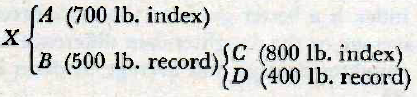
\includegraphics[width=\textwidth]{Page_375.png}
\end{figure}

\noindent
We would estimate \textit{X} at \(\dfrac{700}{2} + \dfrac{500}{2}\), or
pounds, modified, of course, by whatever allowance toward the breed
average we think is necessary on account of our not being sure that the
information about \textit{A} and \textit{B} is exactly equal to their
breeding values. If \textit{B}'s records are few or made under uncertain
circumstances, we will have less faith in them and will examine her
pedigree. That indicates that she was expected to produce
\(\dfrac{800}{2} + \dfrac{400}{2}\), or 600, instead of the 500 she
actually produced. Hence, we will suspect that she really has a little
better heredity than her own record indicates. We will not be certain
of that because we are not entirely certain of the breeding values of
\textit{C} and of \textit{D} and because all animals are so heterozygous
that such a mating as that of \textit{C} and \textit{D} might produce
an individual much poorer or better than is expected. The amount of
attention we give to \textit{C} and \textit{D} will depend mainly on how
uncertain we are that the 500-pound figure correctly represents \textit{B}'s
inheritance. If \textit{B} were never tested -- for example, if \textit{X}
were her first calf and she had died soon after calving -- we would estimate
\textit{X} at \(\dfrac{700}{2} + \dfrac{800}{4} + \dfrac{400}{4}\), or 650
pounds, modified by some allowance toward the breed average; but we would
be more uncertain about our estimate than if \textit{B} had been tested.
\index{Pedigrees as aids to selection|)}

\section*{SUMMARY}

A sire index is a means of expressing in a single figure a sire's progeny
test, usually for characteristics he cannot express himself. It is
most frequently used for dairy bulls and for roosters.

The index which seems most useful and accurate under many conditions
is the average of his daughters plus the average increase of the
daughters over their dams.

The daughter average and the difference between daughters and
dams are the parts of which the index is the sum. The daughter average
is most vulnerable to error from differences in environment from herd
to herd. The difference between daughters and dams is most vulnerable
to error from environment's not having been the same for daughters
and dams or from the dams' having been selected more highly than is
fully discounted. The difference between daughters and dams is least
subject to error from variations in environment from one herd to
another. The index is a better guide to the sire's breeding value than
the daughter average or the daughter-dam difference when the correlation
between daughter average and average of dams is more than .25
but less than .75.

Some room should still be left for considering the production of
ancestors and collateral relatives, even when a bull has many daughters.
An index cannot be guaranteed correct, since indexes will often contain
considerable error from Mendelian sampling and from incomplete corrections
for other circumstances. Hence a sire should be estimated nearer
the average of the breed than his index is, especially if his index is
extremely high or extremely low.

\section*{REFERENCES}

\begin{hangparas}{0.5in}{1}%
Copeland, Lynn. 1934. Pedigree analysis as a basis of selecting bull calves. Jour.
Dy. Sci., 17:911--102.

Davidson, F. A. 1925. Measuring the breeding value of dairy sires by the records of
their first few advanced registry daughters. Illinois Agr. Exp. Sta., Bul. 270.

Engeler, W. 1934. Die Leistungsverbessernden Stiere in der schweizerischen Braunviehzucht.
Luzern.

Gifford, W. 1930. The mode of inheritance of yearly butterfat production. Missouri
Agr. Exp. Sta., Res. Bui. 144.

Goodale, H. D. 1927. A sire's breeding index with special reference to milk production.
American Naturalist, 61:539--44.

Gowen, John W. 1930. On criteria for breeding capacity in dairy cattle. Proc. of
Amer. Soc. An. Prod. for 1929, pp. 47--49.

Hansson, N. 1913. Kan man med f\"ordel h\"oja meddelfetthalten i den av vora
n\'{o}tkreatursstammar och raser l\"{a}mnade mj\"olken? Centralanst. f\"or
f\"ors\"oksv\"asendet p\AA jordbruksomradet, Meddelande, 78:1--85.

Juli, M. A. 1934. Progeny testing in breeding for egg production. Poultry Sci.
13:44--51.

L\"{o}rtscher, Hans. 1937. Variationsstatistische $\grave{U}$ntersuchungen an
Leistungserhebungen in einer British-Friesian Herde. Zeit. f. Z\"ucht. Reihe B.
39:257--362.

Lush, Jay L. 1931. The number of daughters necessary to prove a sire. Jour. of
Dy Sci., 14:209--20.

---. 1933. The bull index problem in the light of modern genetics. Jour. of
Dy. Sci., 15:501--22.

---. 1935. Progeny test and individual performance as indicators of an animal's
breeding value. Jour. of Dy. Sci., 18:1--19.

---. 1944. The optimum emphasis on dams' records when proving dairy
sires. Jour. of Dy. Sci., 27:937--951.

---, Norton, H. W., III, and Arnold, Floyd. 1941. Effects which selection of
dams may have on sire indexes. Jour. of Dy. Sci., 24:695--721.

Mount Hope Farm. 1928. Selecting a herd sire. The Mount Hope Bull Index. Mount
Hope Farm, Williamstown, Mass.

Rice, V. A. 1944. A new method for indexing dairy bulls. Jour. of Dy. Sci.,
27:921--36.

Turner, C. W. 1925. A comparison of Guernsey sires. Missouri Agr. Exp. Sta., Res.
Bul. 79 (see especially p. 27).

Ward, A. H. 1941. Sire survey and investigational work. Seventeenth annual report
of the New Zealand Dairy Board.

Wright, S. 1932. On the evaluation of dairy sires. Proc. Amer. Soc. An. Prod. for
1931, pp. 71--78.

Yapp, W. W. 1925. Transmitting ability of dairy sires. Proc. Amer. Soc. An. Prod.
for 1924, pp. 90--92.
\end{hangparas}
\index{Sire indexes|)}